\documentclass[conference]{IEEEtran}
\IEEEoverridecommandlockouts

\usepackage{graphicx}
\usepackage{booktabs}
\usepackage{amsmath}
\usepackage{amssymb}
\usepackage{tikz}
\usetikzlibrary{positioning, arrows.meta, calc}
\usepackage{cuted}
\usepackage{capt-of}
\usepackage{cite}
\definecolor{tgperi}{HTML}{5A7AB8}
\definecolor{tgbrown}{HTML}{3B1E1C}
\usepackage[colorlinks=true,citecolor=tgperi,linkcolor=tgperi,urlcolor=tgperi]{hyperref}

\graphicspath{{figures/}}

% Bold run-in heading (IEEEtran's \paragraph renders as lettered 'a)')
\newcommand{\parhead}[1]{\smallskip\noindent\textbf{#1}\hspace{0.6em}}

\begin{document}

\title{FieldVote: Consensus Polygonization for Field Boundaries}

\author{
\IEEEauthorblockN{Aviskar Giri and Isaac Corley}
\IEEEauthorblockA{Taylor Geospatial, St.\ Louis, MO, USA\\
aviskar.giri@taylorgeospatial.org}
}

\maketitle

\begin{strip}
\centering
\begin{tikzpicture}[>={Latex[length=2mm]}, font=\footnotesize,
  img/.style={inner sep=0pt, outer sep=0pt},
  plbl/.style={font=\scriptsize, align=center},
  pbox/.style={draw=tgbrown, rounded corners, fill=tgperi!15, align=center, font=\footnotesize, inner sep=3pt},
  flow/.style={->, semithick, tgbrown!75}]
  \node[img] (in) {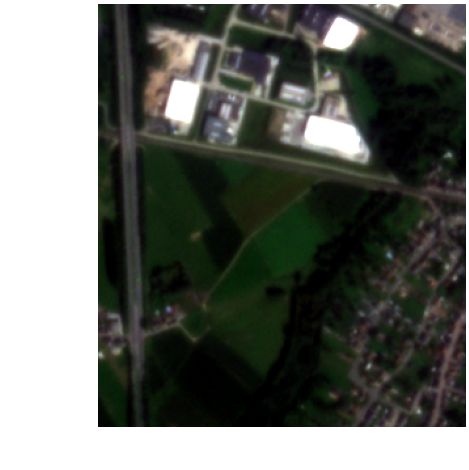
\includegraphics[width=0.12\textwidth]{fig_pipe_input.png}};
  \node[plbl,below=0.5mm of in] {Input tile};
  \node[pbox,right=7mm of in] (net) {Frozen\\net};
  \node[img, right=7mm of net] (prob) {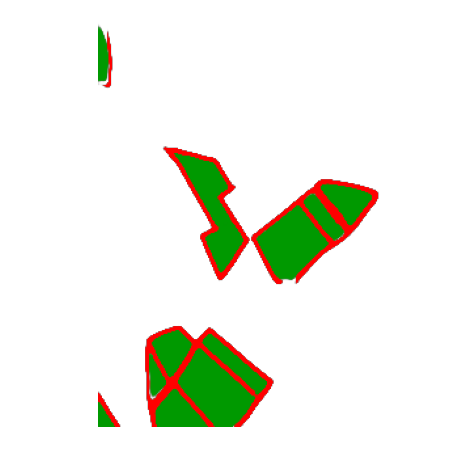
\includegraphics[width=0.12\textwidth]{fig_pipe_prob.png}};
  \node[plbl,below=0.5mm of prob] {Field and boundary\\probability};
  \node[img, above right=3mm and 12mm of prob] (wlow) {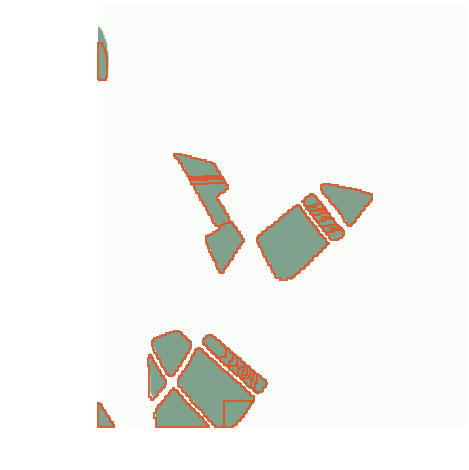
\includegraphics[width=0.10\textwidth]{fig_pipe_wslow.png}};
  \node[plbl,above=0.5mm of wlow] {low $h$, over-split};
  \node[img, below right=3mm and 12mm of prob] (whigh) {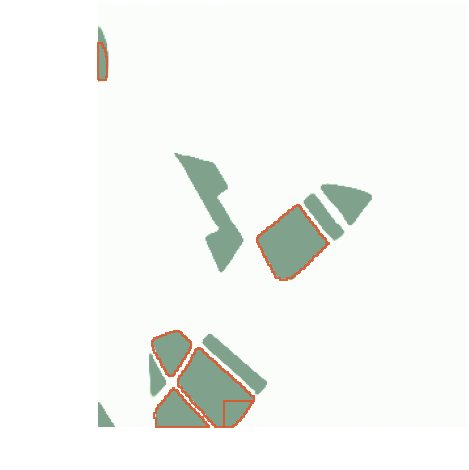
\includegraphics[width=0.10\textwidth]{fig_pipe_wshigh.png}};
  \node[plbl,below=0.5mm of whigh] {high $h$, merged};
  \coordinate (wmid) at ($(wlow.east)!0.5!(whigh.east)$);
  \node[pbox,right=10mm of wmid] (vote) {Per-pixel\\majority vote};
  \node[img, above right=3mm and 12mm of vote] (cons) {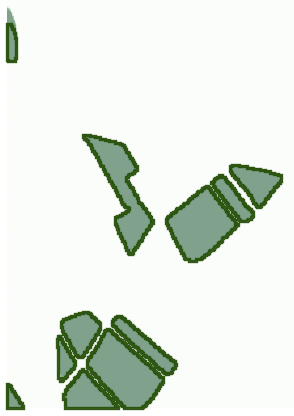
\includegraphics[width=0.10\textwidth]{fig_pipe_consensus.png}};
  \node[plbl,above=0.5mm of cons] {Consensus};
  \node[img, below right=3mm and 12mm of vote] (agr) {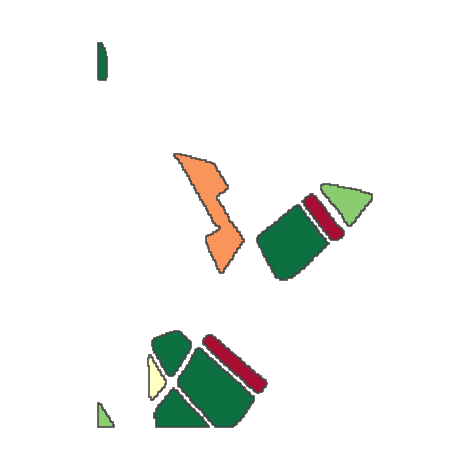
\includegraphics[width=0.10\textwidth]{fig_pipe_agreement.png}};
  \node[plbl,below=0.5mm of agr] {Agreement};
  \node[img, right=9mm of cons] (gt) {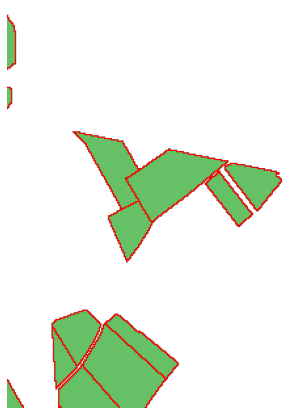
\includegraphics[width=0.10\textwidth]{fig_pipe_gt.png}};
  \node[plbl,above=0.5mm of gt] {Ground truth};
  \draw[flow] (in) -- (net);
  \draw[flow] (net) -- (prob);
  \draw[flow] (prob.east) -- (wlow.west);
  \draw[flow] (prob.east) -- (whigh.west);
  \draw[flow] (wlow.east) -- (vote.west);
  \draw[flow] (whigh.east) -- (vote.west);
  \draw[flow] (vote.east) -- (cons.west);
  \draw[flow] (vote.east) -- (agr.west);
  \draw[dashed, semithick, tgbrown!55] (cons.east) -- node[above=-1pt, font=\scriptsize, text=tgbrown]{$\approx$} (gt.west);
\end{tikzpicture}
\captionof{figure}{\textbf{FieldVote} on a held-out Belgium tile. A frozen network maps the input tile to a field and boundary probability map, and we change only the steps that follow. The watershed runs at many h-minima thresholds: a low threshold over-segments the fields into 44 fragments (thin internal splits) and a high threshold merges neighbors. A per-pixel majority vote keeps only the boundaries that recur across the sweep, giving 11 consensus polygons. The same vote produces a label-free per-field agreement score (green high, red low) that flags uncertain fields, and the consensus closely matches the ground-truth annotation (right).}
\label{fig:pipeline}
\end{strip}

\begin{abstract}
Per-pixel field-boundary segmentation models produce probability maps, but downstream users need polygons. The conversion step between the two largely determines the accuracy of the delivered product. We study that conversion for a frozen UNet with an EfficientNet-B7 encoder. We retrain nothing and change only how its per-pixel field and boundary probabilities become field polygons. We evaluate with polygon-level metrics, led by Panoptic Quality, on the Fields of The World benchmark, a smallholder subset, and across Sentinel-2 and PlanetScope imagery. Our main finding is that no single watershed threshold works across regions. FieldVote runs the watershed at many h-minima thresholds and takes a per-pixel majority vote over the resulting segmentations. It reaches a macro PQ of 35.8 over the held-out test splits of the ten dense-label countries. This matches the trained-model PlanetScope headline with a frozen model and no retraining, and it improves over a per-country tuned watershed (29.0) by a statistically significant margin (Wilcoxon $p = 0.049$). The vote also yields a label-free per-field confidence score that predicts per-field accuracy within a region. Applied to the global Fields of The World Sentinel-2 prediction store, FieldVote runs unchanged across sensors and continents, and the agreement signal indicates where it helps. We also report negative results. Geometric refinement designed for buildings does not help organic field boundaries. Regularization and corner smoothing each move mean PQ by at most 0.2 over 23 countries, and the regularization gain shows no significant association with field rectangularity ($r = 0.135$, $p = 0.55$). Douglas--Peucker simplification cuts vertices per polygon sixteen-fold while PQ falls only 0.5. Of the postprocessing steps we tested, FieldVote is the only one that improves the metric.
\end{abstract}

\begin{IEEEkeywords}
field boundary delineation, postprocessing, instance segmentation, watershed, panoptic quality, remote sensing
\end{IEEEkeywords}

\section{Introduction}
Field boundaries are the unit of analysis for crop monitoring, yield estimation, subsidy administration, and land-use accounting. Mapping them at continental scale requires automated delineation from satellite imagery. The dominant approach trains a convolutional network to predict, for every pixel, the probability of field interior and of field boundary~\cite{kerner2024ftw,waldner2020decode}. These probability maps are accurate and well studied, but a cadastre, a yield model, or a subsidy auditor consumes vector polygons rather than rasters of class scores. The step that converts probabilities into polygons therefore determines the quality of every downstream product, and it is the step we study here.

Pixel-level metrics such as intersection over union reward correct labeling of large interior regions and are nearly insensitive to whether two adjacent fields are separated. Since the object of interest is the field, the metric should be object-level. We lead with Panoptic Quality~\cite{kirillov2019panoptic}, which factors as segmentation quality times recognition quality (PQ = SQ $\times$ RQ) and penalizes both merged and fragmented fields, complemented by Boundary IoU~\cite{cheng2021boundaryiou} and average precision. Under these metrics a model with high pixel accuracy can still produce unusable polygons (Fig.~\ref{fig:qualitative}). Vectorization has received far less attention than the network, and we find it is where the remaining accuracy sits.

Converting a boundary probability map into polygons is classically done by watershed segmentation seeded at suppressed minima~\cite{soille2004morphological,koyuncu2016iterative,waldner2020decode}. The result depends sharply on the h-minima suppression threshold. A low threshold over-fragments large fields and a high threshold merges small ones, and no single value is correct across countries. Values suited to the large rectangular fields of northern Europe over-fragment the small irregular fields of smallholder regions, and values suited to smallholder regions merge large fields into blobs. Field geometry compounds the difficulty. Agricultural parcels are organic rather than rectilinear, so geometric priors imported from building extraction~\cite{zorzi2022polyworld,girard2021framefield,zorzi2020regularization} do not transfer. Ground-truth polygons are also expensive, so any improvement must work without per-region labels for tuning.

Model accuracy varies widely by country~\cite{kerner2024ftw,corley_ftp,ftw_global}, yet a practitioner rarely cares about the global average. They map their own country or a small area of interest and need good boundaries there. Tuning the watershed threshold per region would demand ground-truth polygons in every new area, which do not exist at scale, and a single globally tuned threshold is a compromise that suits no region in particular. What a user needs is one label-free postprocessing rule, with one fixed set of hyperparameters, that performs well across regions without per-region calibration. FieldVote is such a rule.

We change nothing about the network. We treat its frozen probability maps as fixed inputs and study only the conversion to polygons, which isolates the contribution of postprocessing and keeps the comparison against the trained-model headline fair. Our main finding is that no single watershed threshold works across regions. We instead run the watershed at many thresholds and take a per-pixel majority vote over the resulting segmentations. FieldVote reaches a macro PQ of 35.8 over the held-out test splits of the ten dense-label countries, matching the trained-model PlanetScope headline, while a per-country tuned watershed reaches 29.0 and the DelineateAnything baseline~\cite{lavreniuk2025delineateanything} reaches 5.0 (14.6 in its strongest configuration). The improvement over the tuned watershed is statistically significant (Wilcoxon $p = 0.049$, bootstrap 95\% confidence interval on the mean gain $[1.2, 12.1]$). FieldVote scores higher where a single threshold over-fragments, for example Belgium (52.9 versus 30.6) and Croatia (35.8 versus 20.5), and lower on the smallest-field smallholder cases (Cambodia, Portugal) and Germany. The same vote agreement yields a label-free per-field confidence score.

We also report negative results, so that others do not repeat the same experiments. Geometric refinement built for buildings does not help organic fields, and soft-boundary watershed is neutral. Simplification compresses geometry but does not improve accuracy. This paper contributes four results. First, FieldVote, a per-pixel majority vote over watershed segmentations run at many h-minima thresholds, reaches macro PQ 35.8 on the held-out test splits of the ten dense-label countries. It matches the trained-model headline with a frozen model, improves on the tuned watershed by a statistically significant margin, and has a size-adaptive variant that further protects small fields. Second, the same threshold-vote agreement gives a label-free per-field confidence that predicts per-field IoU against ground truth within a region (Spearman 0.20 to 0.42, $p < 0.0001$, in 5 of 6 countries). Third, a study of refinement operators shows that building-derived regularization, smoothing, and raster cleanup do not transfer to organic fields, that simplification compresses vertex counts sixteen-fold at little accuracy cost, and that soft-boundary watershed is neutral. Fourth, we run FieldVote unchanged on the global Fields of The World Sentinel-2 prediction store across eight regions on five continents, to our knowledge the first global-scale evaluation of a field-boundary postprocessing technique, and show that the agreement signal indicates where it helps.

\section{Related Work}
\parhead{Field-boundary delineation and watershed postprocessing.}
Field delineation is commonly cast as dense prediction of a field and boundary map followed by instance extraction. Waldner and Diakogiannis~\cite{waldner2020decode} predict extent, boundary, and distance with a FracTAL ResUNet and recover parcels by seeded watershed, establishing the encoder-then-watershed pipeline that the Fields of The World benchmark~\cite{kerner2024ftw} adopts. The watershed is classical morphology~\cite{soille2004morphological} that floods a surface from markers, and the choice of markers governs whether parcels merge or fragment. Koyuncu et al.~\cite{koyuncu2016iterative} make marker selection explicit by sweeping the h-minima depth and iterating, which exposes over-segmentation and under-segmentation as a single tunable axis. Wagner and Oppelt~\cite{wagner2020growing} drive a hierarchical watershed from learned contours under Sentinel-2 resolution. These methods fix one operating point per scene. We instead retain the full h-minima sweep and combine its outputs.

\parhead{Learned versus geometric polygon extraction.}
A second line extracts polygons directly. Girard et al.~\cite{girard2021framefield} learn a frame field aligned to parcel geometry and report that downstream Douglas--Peucker simplification lowers AP. PolyWorld~\cite{zorzi2022polyworld} predicts vertices and connectivity as a graph. Geometric refinement matured on buildings, where right-angle priors hold. Zorzi et al.~\cite{zorzi2020regularization} regularize masks with an adversarial network that imposes rectilinear outlines. We test whether these building-oriented operators transfer to organic fields and find that they do not.

\parhead{Non-maximum suppression, ensembling, and consensus.}
Our per-pixel vote is most directly inspired by non-maximum suppression (NMS), the standard object-detection postprocessing that keeps confident detections and suppresses overlapping spurious ones~\cite{neubeck2006nms}. Modern variants soften or learn this rule: Soft-NMS decays overlapping scores rather than removing them~\cite{bodla2017softnms}, Learning-NMS replaces the hand-set rule with a network~\cite{hosang2017learningnms}, and Weighted Boxes Fusion combines detections from several models by agreement~\cite{solovyev2021wbf}. FieldVote applies the same principle at the pixel level and across an operating-parameter sweep rather than across models. A boundary that recurs across watershed thresholds is kept, and one that appears at a single threshold is suppressed. Deep ensembles~\cite{lakshminarayanan2017deepensembles}, MC dropout~\cite{gal2016dropout}, and test-time augmentation~\cite{wang2019tta} aggregate multiple predictions, but they retrain or re-infer the network. We instead aggregate over a postprocessing hyperparameter of a single frozen model, which acts as a stability filter. The same view frames our baseline. DelineateAnything~\cite{lavreniuk2025delineateanything} is an instance-segmentation model that already applies NMS to its own predictions, so comparing against it sets one postprocessing pipeline against another rather than against a raw model.

\parhead{Evaluation metrics.}
We lead with object-level metrics because pixel accuracy tolerates merged or split parcels. Panoptic Quality~\cite{kirillov2019panoptic} penalizes both localization and instance-count error, and we complement it with Boundary IoU~\cite{cheng2021boundaryiou}. This object-first protocol matches recent smallholder and pan-European benchmarks~\cite{persello2023ai4smallfarms,dandrimont2023ai4boundaries} and the Fields of The World~\cite{kerner2024ftw} and Fields of the Planet~\cite{corley_ftp} evaluations.

\begin{figure}[t]
\centering
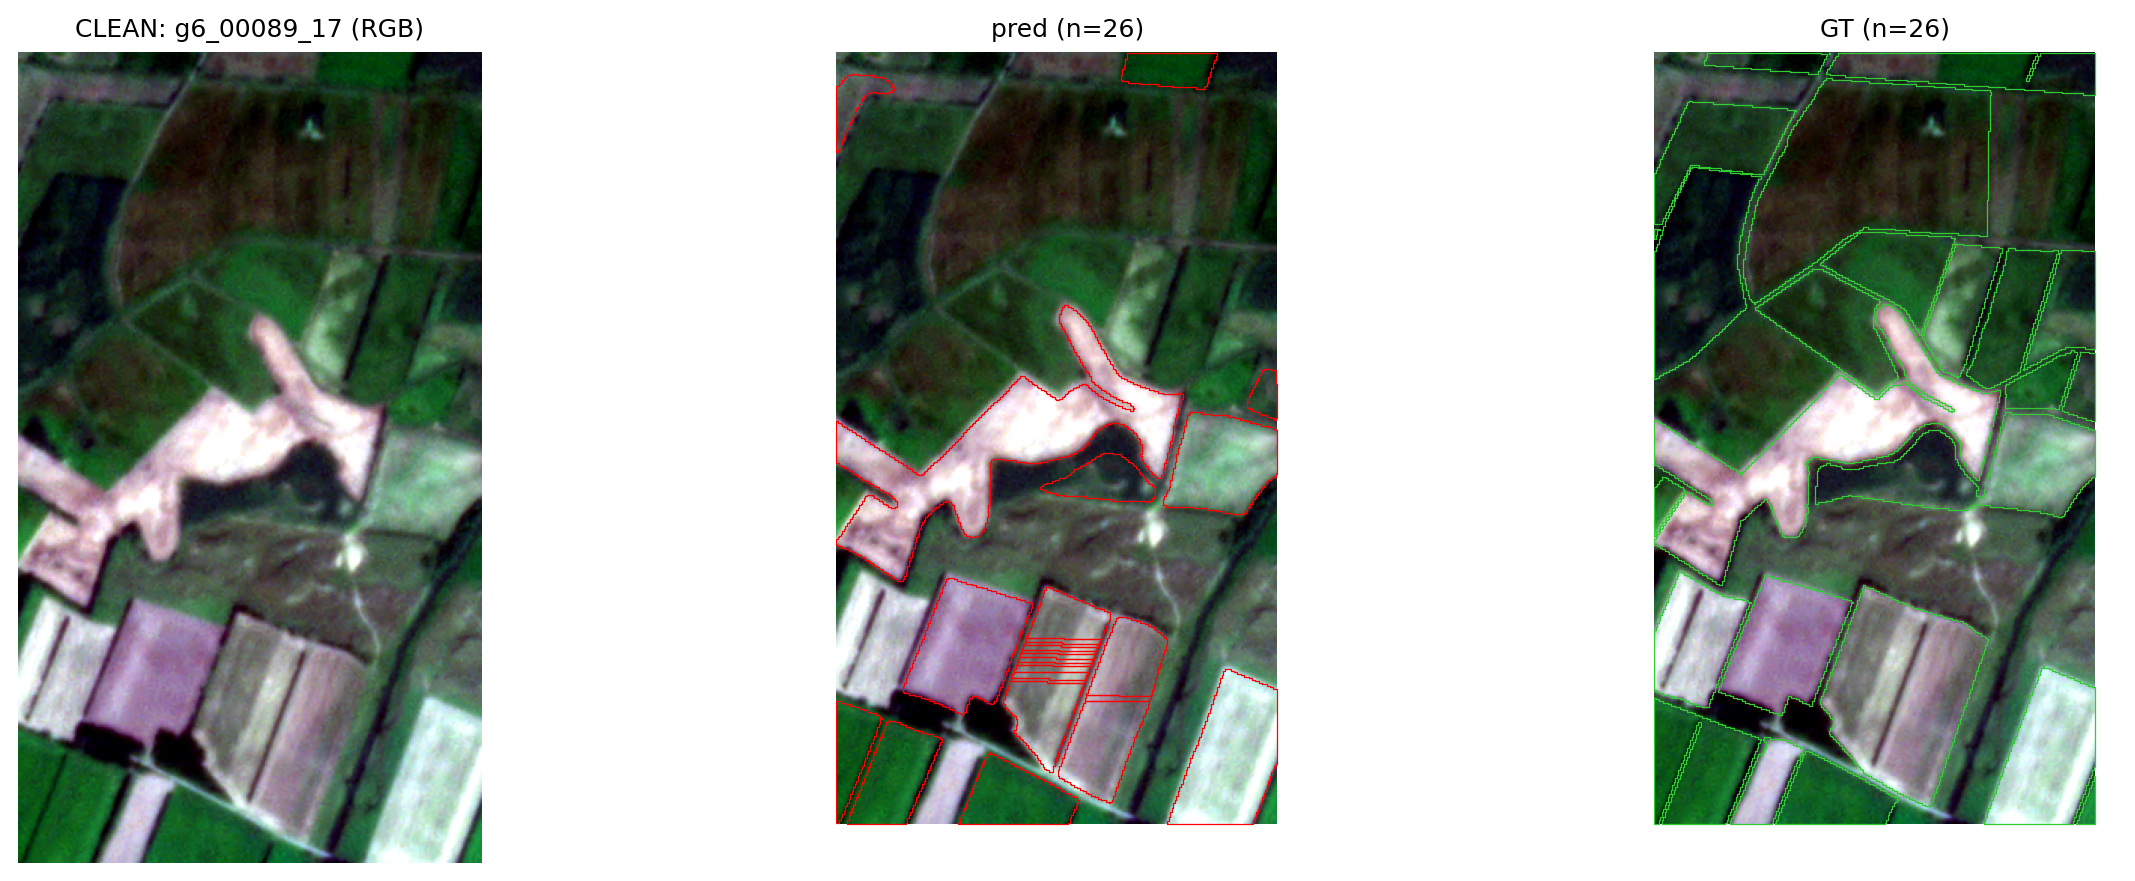
\includegraphics[width=\columnwidth]{qualitative_example.png}
\caption{An example held-out patch (left), the field polygons FieldVote produces from the frozen model (center), and the ground-truth boundaries (right). Instance counts appear above each panel. Object-level quality depends on matching the number and shape of parcels, which pixel accuracy alone does not capture.}
\label{fig:qualitative}
\end{figure}

\section{Method}
\label{sec:method}
We postprocess a frozen UNet with an EfficientNet-B7 encoder that produces a per-pixel softmax over field interior, boundary, and background. We hold the weights fixed and replace only the conversion of these probabilities into polygons (Fig.~\ref{fig:pipeline}).

\subsection{Threshold-consensus polygonization}
\label{sec:consensus}
Marker-controlled watershed seeds from regional minima after an h-minima transform that suppresses minima shallower than a depth $h$~\cite{koyuncu2016iterative,waldner2020decode}. The choice of $h$ governs fragmentation, and a single $h$ fixes one point on the over-segmentation versus under-segmentation trade-off for an entire region. We run the watershed independently at each threshold in a fixed set $H = \{h_1, \dots, h_K\}$. Run $k$ yields a label map $L_k$, which we convert to a per-pixel field indicator. Writing the per-pixel vote fraction as
\begin{equation}
\bar{f}(p) = \frac{1}{K}\sum_{k=1}^{K}\mathbb{1}[p \in \text{field in } L_k],
\label{eq:vote}
\end{equation}
the consensus assigns a pixel to field when $\bar{f}(p) \geq \tau_v$, with the majority vote $\tau_v = 0.5$. We polygonize the connected components of the consensus mask. This rule keeps a field only where it is stable across the sweep. Spurious splits at a single shallow $h$ are voted down, and divisions that recur across the range are retained. The procedure adds no learned parameters. Equivalently, $\bar{f}(p)$ is a per-pixel agreement score, and assigning field where $\bar{f}(p)\geq\tau_v$ is the spatial analogue of non-maximum suppression, which retains only detections whose agreement exceeds a threshold~\cite{neubeck2006nms,solovyev2021wbf}. The per-country tuned watershed is the degenerate case $K=1$, with $\bar{f}(p)=\mathbb{1}[p\in\text{field in }L_{h^\star}]$ for a single tuned depth $h^\star$. The consensus recovers the cross-threshold agreement that one operating point discards. Figure~\ref{fig:pipeline} shows the full procedure on a held-out tile, from the probability map through the per-threshold watershed segmentations to the consensus polygons and the agreement score.

\subsection{Geometric refinement and raster cleanup}
\label{sec:geometric}
We test whether refinement operators developed for buildings transfer to fields, applying four stages to the polygon output: Douglas--Peucker simplification; rectilinear edge regularization that snaps edges toward dominant orientations~\cite{zorzi2020regularization}; Chaikin corner-cutting smoothing; and a morphological raster cleanup (small-component removal and hole filling) applied before the watershed.

\subsection{Threshold-agreement confidence}
\label{sec:confidence}
The sweep also supplies a label-free confidence score. For a consensus field $F$ we define its agreement as the fraction of the $K$ runs whose label map contains a basin overlapping $F$ with intersection over union at least $\theta$,
\begin{equation}
a(F) = \frac{1}{K}\sum_{k=1}^{K}\mathbb{1}\!\left[\exists\, c \in L_k : \mathrm{IoU}(c, F) \geq \theta\right].
\label{eq:agree}
\end{equation}
We set the matching threshold $\theta = 0.5$. A field delineated identically at every threshold scores $a(F)=1$, and because $a(F)$ needs no ground truth, it is available wherever the model runs.

\subsection{Size-adaptive consensus}
\label{sec:adaptive}
The uniform majority vote helps where fields are large and clean, but it can over-merge where they are small and dense. We therefore choose the rule per patch using a label-free signal, the mean area of the vote-consensus instances. Below a size threshold $T$ we blend the vote with the field probability ($0.4\,\bar{f} + 0.6\,p_{\text{field}} \geq 0.5$), and otherwise we keep the pure vote. The switch needs no labels and adds one parameter $T$.

\section{Experimental Setup}
\label{sec:setup}
We postprocess one frozen UNet with an EfficientNet-B7 encoder, the PlanetScope model of Corley et al.~\cite{corley_ftp} trained on Fields of The World~\cite{kerner2024ftw}, and operate only on its stored softmax, so every comparison isolates the polygonization step. We report two scopes. The headline polygon-quality comparison uses the held-out test splits of the ten dense-label countries (\textsc{Dense-10}). We exclude Kenya, the only presence-only region, whose unlabeled background makes supervised polygon metrics unreliable~\cite{kerner2024ftw}. The geometric-refinement study uses the 23 countries for which the full polygon stack was scored, and the confidence and soft-boundary studies use the subset for which per-pixel probabilities were stored. These counts reflect data availability rather than selection. Baselines are the trained-model PlanetScope headline~\cite{corley_ftp}, a per-country tuned watershed (the best single h-minima threshold selected per country), and DelineateAnything~\cite{lavreniuk2025delineateanything} run on the same imagery in both its default and strongest configurations. Following the polygon-level evaluation protocol of Fields of the Planet~\cite{corley_ftp}, metrics are Panoptic Quality with its SQ and RQ factors~\cite{kirillov2019panoptic}, average precision, Boundary IoU~\cite{cheng2021boundaryiou}, and mean vertex count. All macro numbers are averaged across the relevant countries.

\section{Results}
\label{sec:results}

\parhead{FieldVote matches the trained-model headline.}
Table~\ref{tab:headline} reports macro PQ on \textsc{Dense-10}. FieldVote reaches 35.8 with a frozen model and no retraining, matching the trained-model PlanetScope headline. On the same EfficientNet-B7 backbone the trained model scores 35.4, and its EfficientNet-B3 headline scores 35.5, the two being effectively tied~\cite{corley_ftp}. FieldVote also improves on the per-country tuned watershed by 6.8. This gain is statistically significant across countries (Wilcoxon signed-rank $p = 0.049$; bootstrap 95\% confidence interval on the mean gain $[1.2, 12.1]$). DelineateAnything trails both by a wide margin (Table~\ref{tab:headline}). FieldVote therefore recovers the trained-model polygon quality by aggregating operating points of the existing softmax. The gain is not confined to PQ. FieldVote also leads the tuned watershed on segmentation quality, recognition quality, average precision, and Boundary IoU~\cite{cheng2021boundaryiou} (Table~\ref{tab:metrics}). The headline also holds under a different ground-truth footing. Scored directly against the released per-patch vector polygons, FieldVote reaches 35.5 versus 28.6 for the tuned watershed, and the gain persists on a stricter instance-mask footing (Appendix~\ref{app:footing}).
% FTP comparator cited (corley_ftp, arXiv 2607.04449). Backbone: trained B7 = 35.4, B3 = 35.5 (tied); we postprocess B7. FOOTING RESOLVED 2026-07-16: the released FTP eval (ftw-planet repo, src/ftw_planet/eval.py) extracts GT shapes from the rasterized semantic mask (gt==1 connected components), the SAME footing as our headline scorer, so 35.8 vs 35.4 is a like-for-like comparison as published. The per-patch GT vector polygons are now public (HF taylor-geospatial/ftw-planet, <pid>.polygons.parquet per patch); a vector-GT re-score is an optional robustness check, not a gate.

\begin{table}[t]
\centering
\caption{Macro PQ (0--100) on \textsc{Dense-10}, the held-out test splits of the ten dense-label countries (presence-only Kenya excluded). FieldVote matches the trained PlanetScope model while retraining nothing and improves on a per-country tuned watershed by 6.8 points, and the learned DelineateAnything baseline trails by more than 20 points. FieldVote and the trained model share the EfficientNet-B7 backbone. The B3 headline of Corley et al.~\cite{corley_ftp} is 35.5, effectively tied with B7. Best in \textbf{bold}.}
\label{tab:headline}
\begin{tabular}{lc}
\toprule
Method & Macro PQ \\
\midrule
DelineateAnything, default~\cite{lavreniuk2025delineateanything} & 5.0 \\
DelineateAnything, strongest~\cite{lavreniuk2025delineateanything} & 14.6 \\
Tuned watershed & 29.0 \\
Trained PlanetScope model, B7~\cite{corley_ftp} & 35.4 \\
\textbf{FieldVote (ours), B7} & \textbf{35.8} \\
\bottomrule
\end{tabular}
\end{table}

\begin{table}[t]
\centering
\caption{Polygon-level metrics on \textsc{Dense-10} (0--100), FieldVote versus the per-country tuned watershed. FieldVote leads on every matching-based metric, namely Panoptic Quality, its SQ and RQ factors, average precision, and Boundary IoU. Macro PQ is the mean of per-country PQ, so it is not exactly SQ$\times$RQ of these row averages. Best in \textbf{bold}.}
\label{tab:metrics}
\begin{tabular}{lccccc}
\toprule
Method & PQ & SQ & RQ & AP & B-IoU \\
\midrule
Tuned watershed & 29.0 & 77.0 & 36.6 & 23.2 & 15.6 \\
\textbf{FieldVote (ours)} & \textbf{35.8} & \textbf{77.7} & \textbf{44.6} & \textbf{29.2} & \textbf{15.9} \\
\bottomrule
\end{tabular}
\end{table}

\begin{figure}[t]
\centering
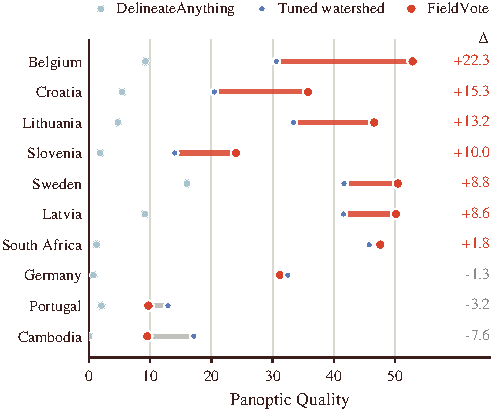
\includegraphics[width=\columnwidth]{fig_percountry.pdf}
\caption{Per-country PQ (0--100) on \textsc{Dense-10}. FieldVote scores higher wherever a single watershed threshold over-fragments, most in the mid-to-large field regimes of Belgium and Croatia, and scores lower only on the smallest-field smallholder cases (Cambodia, Portugal) and Germany. The aggregate gain comes from suppressing spurious splits rather than from uniform improvement.}
\label{fig:percountry}
\end{figure}

Figure~\ref{fig:percountry} shows the per-country breakdown. The aggregate gain comes from suppressing spurious splits in mid-to-large field regimes rather than from uniform improvement. Kenya is excluded from every macro for the presence-only reason given in Section~\ref{sec:setup}. Figure~\ref{fig:results} shows the effect qualitatively on held-out tiles. A single watershed threshold breaks each scene into dozens of fragments, while FieldVote recovers clean parcels that track the ground-truth annotation.

\begin{figure*}[t]
\centering
\footnotesize
\setlength{\tabcolsep}{1.5pt}
\renewcommand{\arraystretch}{0.4}
\begin{tabular}{@{}c@{\ }ccccc@{}}
 & Window A & Window B & Single $h$ & FieldVote (ours) & Ground truth \\
\rotatebox{90}{\enspace Belgium} &
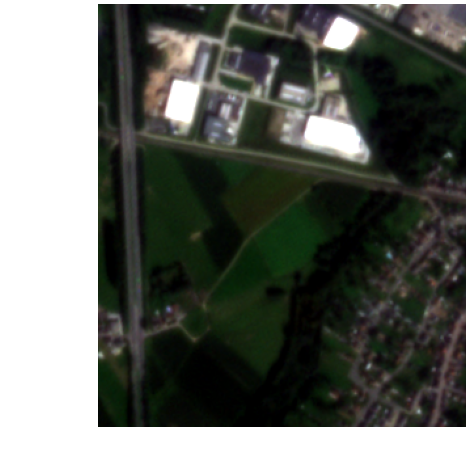
\includegraphics[width=0.18\textwidth]{fig_res_be_in.png} &
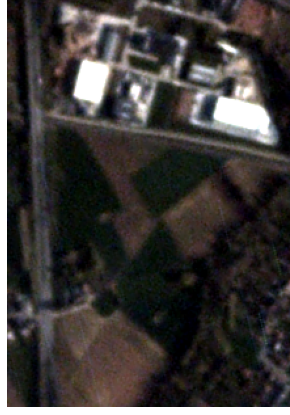
\includegraphics[width=0.18\textwidth]{fig_res_be_inb.png} &
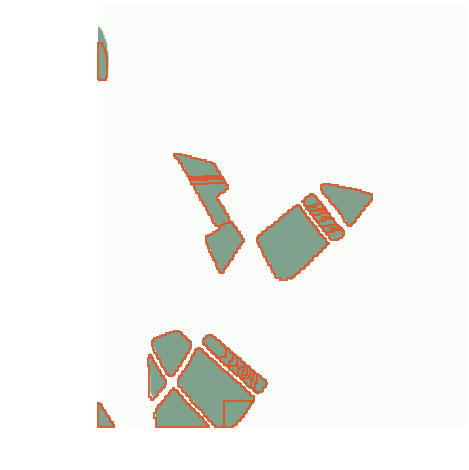
\includegraphics[width=0.18\textwidth]{fig_res_be_single.png} &
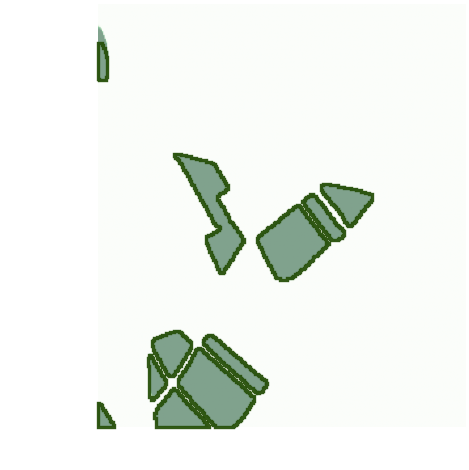
\includegraphics[width=0.18\textwidth]{fig_res_be_fv.png} &
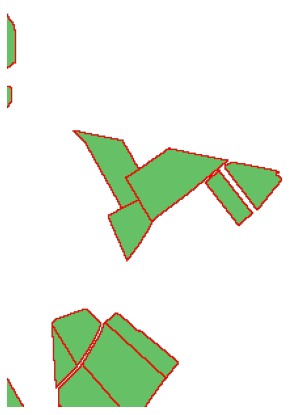
\includegraphics[width=0.18\textwidth]{fig_res_be_gt.png} \\
\rotatebox{90}{\enspace Sweden} &
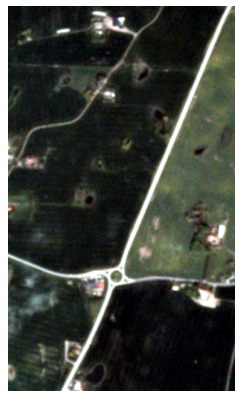
\includegraphics[width=0.18\textwidth]{fig_res_se_in.png} &
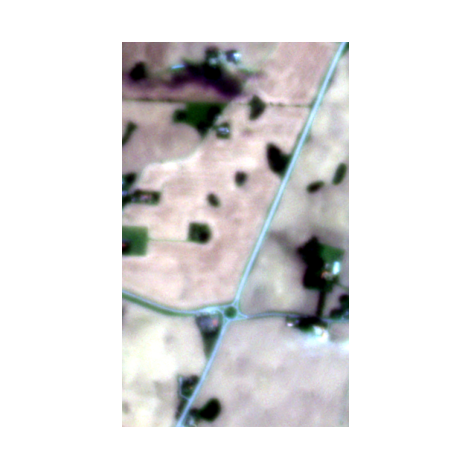
\includegraphics[width=0.18\textwidth]{fig_res_se_inb.png} &
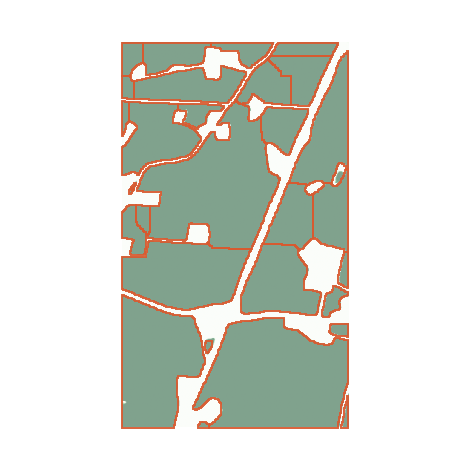
\includegraphics[width=0.18\textwidth]{fig_res_se_single.png} &
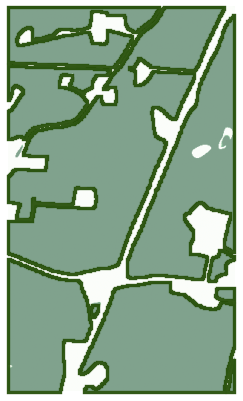
\includegraphics[width=0.18\textwidth]{fig_res_se_fv.png} &
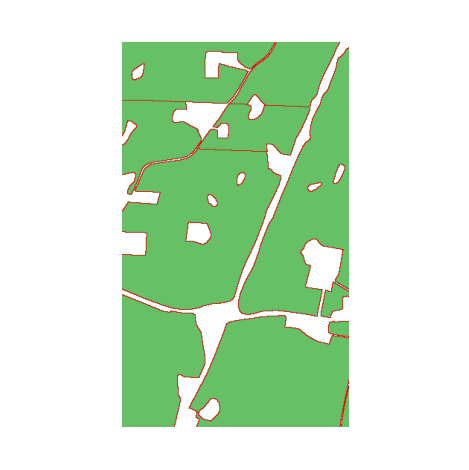
\includegraphics[width=0.18\textwidth]{fig_res_se_gt.png} \\
\rotatebox{90}{\enspace Lithuania} &
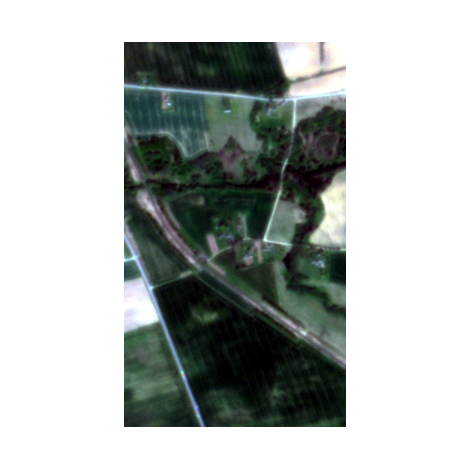
\includegraphics[width=0.18\textwidth]{fig_res_lt_in.png} &
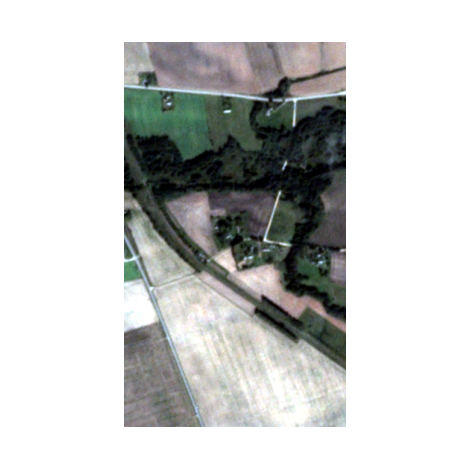
\includegraphics[width=0.18\textwidth]{fig_res_lt_inb.png} &
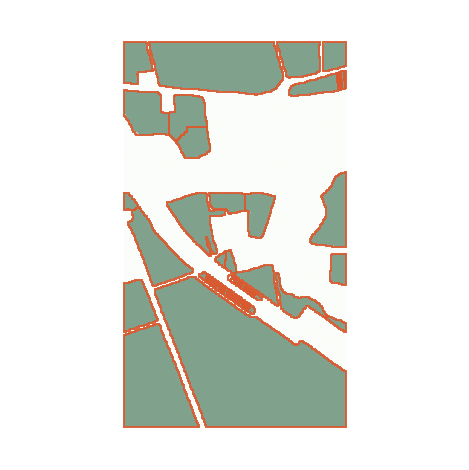
\includegraphics[width=0.18\textwidth]{fig_res_lt_single.png} &
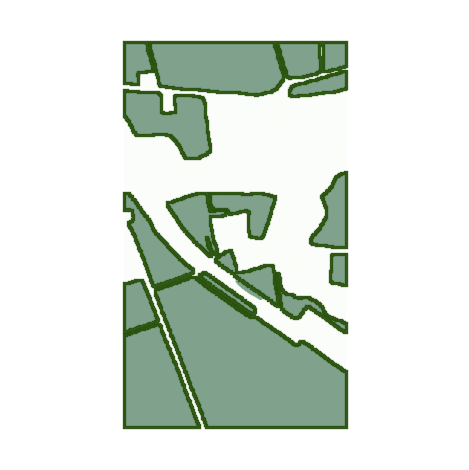
\includegraphics[width=0.18\textwidth]{fig_res_lt_fv.png} &
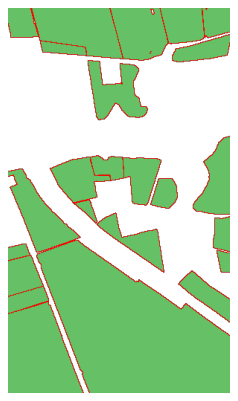
\includegraphics[width=0.18\textwidth]{fig_res_lt_gt.png} \\
\end{tabular}
\caption{FieldVote on three held-out tiles (Belgium, Sweden, Lithuania). Left to right: the two temporal input windows (planting and harvest), watershed at a single low threshold, the FieldVote consensus, and the ground-truth field and boundary annotation. A single operating point over-fragments each scene into dozens of pieces, for example splitting the Lithuania tile into 91. The per-pixel vote keeps only the boundaries that recur across the sweep and recovers 17 parcels for that tile, which track the ground truth without retraining or labels.}
\label{fig:results}
\end{figure*}

\parhead{A size-adaptive rule recovers smallholder accuracy.}
The blend of vote and field probability helps small or fragmented fields but hurts large clean ones, so on its own it ties the uniform vote. Choosing between the two per patch by field size (Section~\ref{sec:adaptive}) captures both cases. On a controlled softmax-derived pipeline the size-adaptive rule raises macro PQ from 33.4 for the uniform vote to 35.2, with $T$ between 50{,}000 and 100{,}000~m\textsuperscript{2}. It recovers the gains on the smallholder and over-fragmenting countries (Belgium, Croatia, Slovenia, Lithuania) without losing the large-field countries (Germany, South Africa, Sweden), as Figure~\ref{fig:adaptive} shows. This pipeline rebuilds instances from the stored softmax rather than the original polygons, so its uniform-vote baseline sits a few points below the polygon headline of Section~\ref{sec:consensus}. We therefore report the size-adaptive result as a relative gain over the uniform vote on identical footing, not as a new absolute headline.

\begin{figure}[t]
\centering
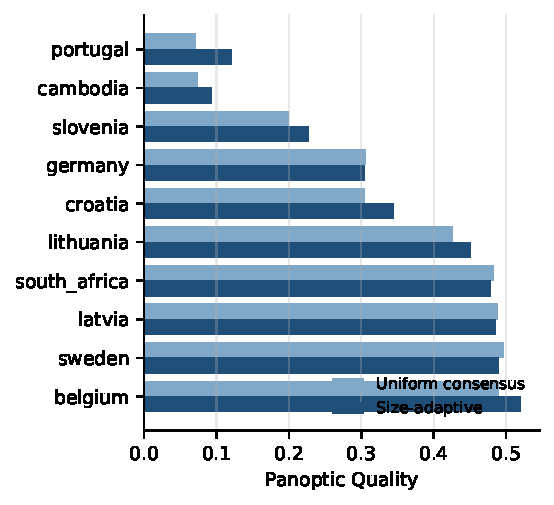
\includegraphics[width=0.85\columnwidth]{fig_adaptive.pdf}
\caption{Size-adaptive FieldVote versus the uniform vote, per country. The adaptive rule matches the uniform vote on large-field countries and improves the small-field and over-fragmenting ones, raising the macro from 33.4 to 35.2 on the same softmax pipeline. The gain is concentrated where the uniform vote over-merges smallholder parcels.}
\label{fig:adaptive}
\end{figure}

\parhead{Geometric refinement does not help organic fields.}
Refinements designed for built structures do not transfer (Table~\ref{tab:refine}). Over 23 countries, no variant improves on raw polygons. Simplification, building-style regularization, and Chaikin smoothing each move mean PQ by at most 0.2. Regularization helps only 1 of the 23 countries, and raster cleanup, evaluated on the 25 countries where it applies, helps only 3 of them. The per-country regularization change shows no significant association with field rectangularity (Pearson $r = 0.135$, $p = 0.55$, $n = 22$), which is consistent with rectilinear priors carrying no useful signal for organic fields. Three further ablations appear in the appendix. The vote threshold is stable around the majority point, Douglas--Peucker simplification compresses vertex counts sixteen-fold at little cost, and soft-boundary watershed is neutral.

\begin{table}[t]
\centering
\caption{Mean PQ (0--100) over 23 countries for post-vectorization geometric refinement. No building-derived operator improves on the raw FieldVote polygons, and each moves the mean by at most 0.2 point. Rectilinear priors that help buildings do not transfer to organic field boundaries.}
\label{tab:refine}
\begin{tabular}{lcc}
\toprule
Variant & Mean PQ & Countries improved \\
\midrule
Raw & 26.5 & -- \\
Simplify (Douglas--Peucker) & 26.4 & -- \\
Regularize (building-style) & 26.3 & 1 / 23 \\
Smooth (Chaikin) & 26.3 & -- \\
\bottomrule
\end{tabular}
\end{table}

\parhead{Agreement predicts per-field quality.}
Within a country, higher-agreement fields are more accurate. The per-field Spearman correlation between agreement and IoU against ground truth is positive and significant in 5 of the 6 countries tested, from 0.20 (Cambodia) to 0.42 (Slovenia), all $p < 0.0001$. Only the smallest test set is not significant (Rwanda, 174 fields). Across countries the signal does not rank regions by accuracy, since mean agreement and macro PQ are uncorrelated ($r = 0.07$). Threshold agreement is therefore a within-region quality estimate rather than a cross-region one. Because it needs no labels, it flags unreliable fields at inference time wherever the model runs.

\parhead{Global, cross-sensor demonstration.}
\label{sec:global}
We apply FieldVote to the global Fields of The World Sentinel-2 prediction store, a 10\,m global mosaic of the same three-class softmax. The model that produced those predictions is Sentinel-2 based, so this also tests whether FieldVote, which we developed on a Planet model, transfers across sensors. To our knowledge this is the first evaluation of a field-boundary postprocessing technique at global scale. We process windows spanning eight agricultural regions on five continents (Table~\ref{tab:global}), and FieldVote runs unchanged on the Sentinel-2 store. The same label-free agreement signal governs its effect. In high-agreement regions (Argentina, France, Australia, Brazil; agreement 95 to 99) it de-fragments, for example Argentina from 426 to 172 polygons (Fig.~\ref{fig:global}). In low-agreement regions (Punjab, Heilongjiang, Ethiopia; agreement 16 to 42) the predictions are themselves unstable across thresholds, and FieldVote produces more and smaller polygons. Agreement therefore indicates when to apply FieldVote in deployment. We do not report polygon-level accuracy here, because global ground-truth parcels are not available. Quantifying global accuracy against reference data is future work.

\begin{table}[t]
\centering
\caption{FieldVote on the global Sentinel-2 prediction store, over a 1536$\times$1536 window per region. Polygon counts before (tuned watershed) and after (FieldVote). FieldVote de-fragments where agreement is high and fragments more where it is low, so the label-free agreement score also serves as a deployment indicator.}
\label{tab:global}
\begin{tabular}{lccc}
\toprule
Region & Tuned WS & FieldVote & Agreement (\%) \\
\midrule
Argentina (Pampas) & 426 & 172 & 98.0 \\
France & 416 & 290 & 95.0 \\
Australia (NSW) & 359 & 319 & 97.0 \\
Brazil (Mato Grosso) & 240 & 208 & 99.0 \\
USA (Iowa) & 434 & 498 & 87.0 \\
China (Heilongjiang) & 164 & 355 & 42.0 \\
India (Punjab) & 20 & 152 & 29.0 \\
Ethiopia & 31 & 81 & 16.0 \\
\bottomrule
\end{tabular}
\end{table}

\begin{figure}[t]
\centering
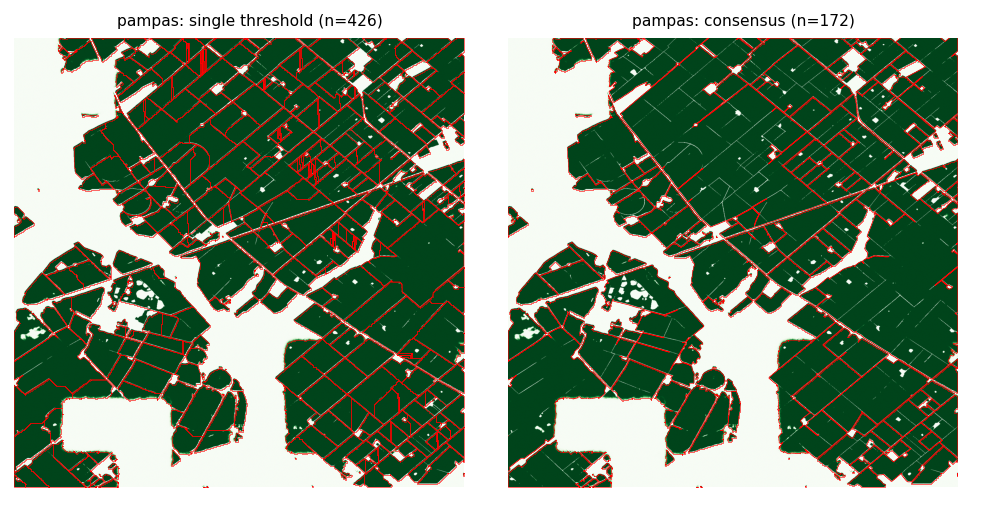
\includegraphics[width=\columnwidth]{global_pampas.png}
\caption{FieldVote on the global Sentinel-2 prediction store, Argentina (Pampas). The field-probability map (green) is overlaid with tuned-watershed polygons (left, $n=426$) and FieldVote polygons (right, $n=172$). In this high-agreement region FieldVote removes spurious splits and recovers coherent parcels, with no labels and no retraining.}
\label{fig:global}
\end{figure}

\section{Discussion}
\parhead{Why the consensus helps.}
The best h-minima depth is not a global constant. It shifts with field size, parcel geometry, and boundary contrast. Choosing a single threshold commits to one point on a sharp trade-off, and the wrong point costs PQ. Rather than selecting a threshold, FieldVote keeps the field boundaries that recur across the sweep, which filters out splits that appear only at shallow depths and merges that appear only at deep depths. The gain is largest in the regions whose best depth lies farthest from the global choice, Belgium (30.6 to 52.9) and Croatia (20.5 to 35.8), where a single threshold over-fragments. For this model and benchmark, better polygonization of a frozen model recovers the trained-model headline. We do not claim this holds for every architecture.

\parhead{Why geometric refinement does not.}
Building regularizers and frame-field polygonizers encode a rectilinear prior~\cite{girard2021framefield,zorzi2022polyworld,zorzi2020regularization} that is correct for buildings and wrong for fields shaped by terrain, hydrology, and incremental division. The absence of a significant rectangularity association is consistent with the prior carrying no useful information for organic boundaries. Simplification is the one geometric operation worth keeping, and it is worth keeping for compression rather than accuracy. Soft-boundary watershed is neutral because the consensus over depths already captures the boundary information that a soft cut exposes.

\parhead{Limitations.}
FieldVote is not uniformly better. It loses on the smallest-field smallholder cases, Cambodia (17.1 to 9.5) and Portugal (12.9 to 9.7), and on Germany (32.5 to 31.2). When fields approach the resolution limit, averaging over thresholds blurs boundaries that are already fragile~\cite{persello2023ai4smallfarms,dandrimont2023ai4boundaries}. The headline gain is a property of medium-to-large parcel landscapes. We postprocess one frozen model, so we cannot separate errors that postprocessing can fix from errors present in the probability map. PQ can also mask systematic boundary displacement that contour metrics would expose~\cite{avbelj2015polis}.

\section{Conclusion}
We treat field-boundary delineation as a polygonization problem on a frozen segmentation model and show that the conversion from probabilities to polygons, rather than the model itself, determines the quality of the resulting parcels. FieldVote, a per-pixel majority vote over watershed segmentations run at many h-minima depths, raises held-out macro PQ from 29.0 to 35.8. It matches the trained-model headline with no retraining, and the gain over the tuned watershed is statistically significant. The same experiments rule out the obvious alternatives. Building-derived geometric refinement does not transfer to organic fields, and soft-boundary watershed is neutral. Simplification is worth applying for its sixteen-fold vertex compression rather than for accuracy. The vote agreement also provides a label-free per-field confidence and, applied to the global Sentinel-2 prediction store, indicates where the consensus transfers across sensors and continents. The method still fails on the smallest smallholder fields. Our size-adaptive variant recovers part of that loss, and extending it into a consensus rule that protects small parcels while retaining the variance reduction that large fields benefit from is the main direction for future work.

\appendices

\section{Vote-threshold sensitivity}
\label{app:vote}
Figure~\ref{fig:vote} sweeps the vote fraction $\tau_v$ from 0.3 to 0.7. Macro PQ is flat across the majority-vote region and declines only when more than 60\% of the thresholds must agree. The majority vote is therefore a near-optimal operating point that we did not have to tune.

\begin{figure}[t]
\centering
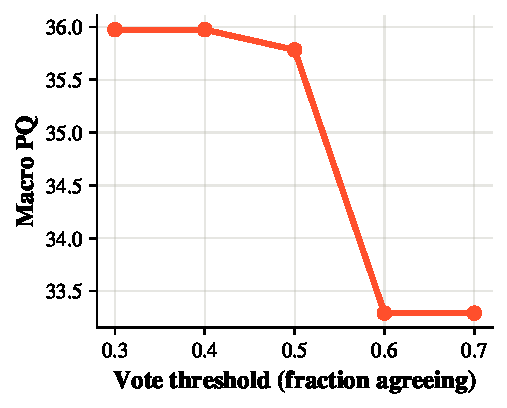
\includegraphics[width=0.85\columnwidth]{fig_votethreshold.pdf}
\caption{Vote-threshold ablation on \textsc{Dense-10}. Macro PQ is flat across the majority-vote region and falls only once more than 60\% of thresholds must agree, so the 0.5 majority vote is a stable operating point rather than a tuned hyperparameter.}
\label{fig:vote}
\end{figure}

\section{Simplification as compression}
\label{app:simplify}
Although simplification does not raise PQ, it compresses geometry at almost no cost (Fig.~\ref{fig:simplify}). As the Douglas--Peucker tolerance grows to 6~m, mean vertices per polygon drop from 188 to 12, a sixteen-fold reduction, while PQ falls only from 36.6 to 36.1. Simplification is worth applying for storage and downstream efficiency, and the choice is independent of the FieldVote gain.

\begin{figure}[t]
\centering
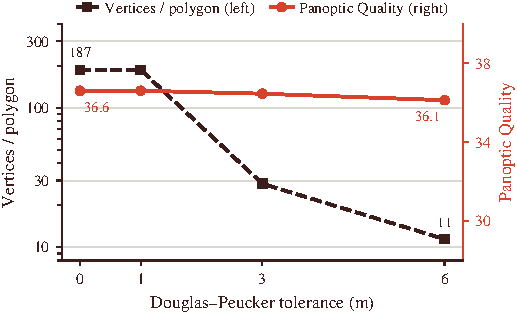
\includegraphics[width=0.85\columnwidth]{fig_simplify.pdf}
\caption{Douglas--Peucker simplification compresses field polygons sixteen-fold (188 to 12 vertices) at small accuracy cost, with PQ falling only from 36.6 to 36.1. Mean over the countries present at every tolerance.}
\label{fig:simplify}
\end{figure}

\section{Soft-boundary watershed is neutral}
\label{app:softboundary}
Thresholding the boundary-class softmax with a swept cut, instead of taking the argmax, changes mean PQ by less than 0.1 across 9 countries and helps 4 of 9, so it is not a useful operation. The consensus over h-minima depths already captures the boundary information that a soft cut exposes.

\section{Ground-truth footing sensitivity}
\label{app:footing}
Polygon metrics depend on how the ground truth itself is represented, so we score both methods on three footings over the same \textsc{Dense-10} test splits (Table~\ref{tab:footing}). The headline footing extracts ground-truth fields as connected components of the rasterized semantic field class, which matches the released Fields of the Planet evaluation protocol~\cite{corley_ftp} and can fuse touching parcels when the separating boundary is lost to rasterization. The instance footing polygonizes per-field instance-id masks projected from the 10\,m label grid onto the 3\,m prediction grid, which prevents fusion but penalizes smooth 3\,m predictions against blocky upsampled edges. The vector footing scores directly against the released per-patch ground-truth polygons, which is the most direct representation. Absolute PQ moves by up to six points across footings, driven almost entirely by the instance footing's resampled edges, and the semantic and vector footings agree within 0.3 points. The FieldVote gain over the tuned watershed is stable on all three, so the paper's conclusion does not depend on the choice of ground-truth representation.

On the vector footing we also report the polygon-count delta of Corley et al.~\cite{corley_ftp}, the mean per-patch $|N_{\text{pred}} - N_{\text{gt}}|$. FieldVote produces the closer count in six of the ten countries, with a mean delta of 8.5 versus 10.8 for the tuned watershed outside the two smallholder countries. The \textsc{Dense-10} macro nevertheless favors the tuned watershed (39.4 versus 61.6) because Cambodia and Portugal dominate it. With roughly 604 and 137 true fields per patch, the consensus merges parcels it cannot separate and undercounts them. This is the same smallholder failure mode discussed in the limitations, and it motivates the size-adaptive variant.

\begin{table}[t]
\centering
\caption{Macro PQ (0--100) on \textsc{Dense-10} under three ground-truth footings. Absolute values shift with the footing, the semantic and vector footings agree closely, and the FieldVote gain is stable throughout.}
\label{tab:footing}
\begin{tabular}{lccc}
\toprule
Footing & FieldVote & Tuned WS & Gain \\
\midrule
Semantic mask (headline) & 35.8 & 29.0 & +6.8 \\
Instance mask & 30.0 & 24.4 & +5.6 \\
Vector polygons & 35.5 & 28.6 & +6.9 \\
\bottomrule
\end{tabular}
\end{table}

\bibliographystyle{IEEEtran}
\bibliography{references}

\end{document}
